% ============================================================================
% Myco-Opt × EO — Extended Abstract for ABOSI4EO Workshop @ AutoML 2026
% Deadline: 14 September 2026 (extended)
% Author: Sebastian Wagner (independent researcher / autodidact)
% ============================================================================
\documentclass[11pt]{article}

\usepackage{microtype}
\usepackage{booktabs}
\usepackage{url}
\usepackage{amsmath}
\usepackage{amssymb}
\usepackage{graphicx}
\usepackage{amsfonts}

% Workshop track: single-blind, no anonymization needed per CFP
\usepackage[workshop,revealauthors]{automl}

\usepackage{natbib}
\bibliographystyle{apalike}

\title{Myco-Opt: Fungal-Network Priors for LLM-Driven Hyperparameter
Optimization in Agricultural Earth Observation}

\author[1]{\nameemail{Sebastián Wagner}{sebastian@wsolutionsai.com}}

\affil[1]{Wagner Solutions AI (independent researcher)}

\hypersetup{%
  pdfauthor={Sebastian Wagner},
  pdftitle={Myco-Opt: Fungal-Network Priors for LLM-Driven HPO in Agricultural EO},
  pdfsubject={AutoML for Earth Observation},
  pdfkeywords={hyperparameter optimization, LLM-as-optimizer, bio-inspired, mycorrhizal networks, Earth Observation, evapotranspiration}
}

\begin{document}

\maketitle

\begin{abstract}
Hyperparameter optimization (HPO) remains sample-inefficient for Earth
Observation (EO) machine-learning pipelines, where each evaluation can involve
training on large multi-spectral time series. Recently, large language models
(LLMs) have been proposed as optimizers (e.g., OPRO), but an unconstrained LLM
proposer explores high-dimensional search spaces poorly when the evaluation
budget is small. We introduce \emph{Myco-Opt}, an LLM-driven HPO framework whose
search space is constrained by \emph{biological priors} extracted from a real
ectomycorrhizal network (Beiler et al., 2010/2015): the same network topology
that evolution shaped to transport water and carbon under uncertainty is used to
shape where an LLM optimizer may search. We evaluate Myco-Opt on an agricultural
EO regression task --- forecasting daily reference evapotranspiration (ET$_0$)
for avocado orchards in La Ligua, Chile, from 10 years of open satellite and
reanalysis data. At a budget of 12 evaluations, the prior improves the LLM
optimizer from RMSE 0.627 (OPRO-vanilla) to 0.614, and Myco-Opt's \emph{first}
proposal (RMSE 0.616) already beats the best configuration the unconstrained
LLM finds in 12 trials (0.621): quantitative biological topology provides a
cheap, transferable prior that makes LLM-based HPO viable in the low-budget
regime that dominates EO practice. All code, data and mappings are open source.
\end{abstract}

\section{Introduction}
\label{sec:intro}

Earth Observation (EO) is a demanding domain for automated ML: modern pipelines
ingest multi-spectral satellite archives, foundation-model embeddings and dense
reanalysis \citep{tuia2021,ruwurm2023}. Finding good hyperparameters is wasteful
when \emph{each} evaluation requires training over long time series; in
operational EO settings the budget is often in the tens, not hundreds, of
trials.

Bayesian optimization (BO, e.g.\ TPE \citep{bergstra2011}) needs many
evaluations to build a reliable surrogate. An alternative casts an LLM as the
optimizer: OPRO \citep{yang2024opro} prompts an LLM with evaluation history to
propose the next configuration --- no surrogate needed. But when the space is
wide and the budget small, an unguided LLM explores poorly: its first proposals
are no better than random.

In this work we ask: \emph{can a quantitative prior derived from real
biological network data make an LLM optimizer competitive in the low-budget
regime?} We answer affirmatively with \textbf{Myco-Opt}, whose search space is
derived from the topology of an ectomycorrhizal network --- the underground
``wood-wide web'' plants use to transport water, carbon and nutrients under
uncertainty \citep{simard1997,beiler2010}. These networks are evolved solutions
to resource-flow optimization under stress; their measured topology provides a
natural prior over the hyperparameters of ML pipelines that must operate under
hydrological stress.

We evaluate Myco-Opt for agricultural EO water management: Chile, the world's
third-largest avocado exporter, faces a structural drought in its central zone,
where ~37{,}000 ha of orchards consume ~9{,}000 m$^3$/ha/year
(CAZALAC-UNESCO). Precision irrigation requires forecasting reference
evapotranspiration (ET$_0$). We forecast daily ET$_0$ one day ahead for La
Ligua (center of the Chilean avocado belt) from 10 years (2016--2026) of open
satellite/reanalysis data. Our contributions: (i)~\textbf{Myco-Opt}, an LLM-driven HPO method whose
search space is constrained by metrics measured on a real, published
mycorrhizal network rather than by heuristics; (ii)~an \textbf{agricultural EO
benchmark} (daily ET$_0$ forecasting for avocado orchards from open EO data,
strict temporal splits, full reproducibility); (iii)~an \textbf{empirical
ablation} showing that at budget 12 the prior improves the identical LLM
optimizer (OPRO-vanilla) substantially, while classical TPE remains the
strongest baseline at this budget (Section~\ref{sec:discussion}).

\section{The biological prior}
\label{sec:prior}

\subsection{Mycorrhizal networks as optimized transport systems}
\label{sec:biology}

Ectomycorrhizal fungi form physical networks connecting the roots of multiple
plants, exchanging water, carbon and nutrients \citep{simard1997}. Shaped by
evolution under drought and resource heterogeneity, common-mycorrhizal networks
(CMNs) empirically exhibit \emph{scale-free} degree distributions (few highly
connected ``hub'' trees), \emph{modular} community structure (guilds
specialized on subsets of hosts), and \emph{small-world} connectivity
\citep{beiler2010,southworth2014}.

Myco-Opt's working hypothesis is modest and falsifiable: \textbf{these
structural features, measured on a real network, define a good region of the
hyperparameter space for ML models that must generalize under environmental
noise}. We claim no fungal ``intelligence''; we claim only that quantitative
network topology provides a useful, transferable prior.

\subsection{Data: the Beiler Douglas-fir CMN}
\label{sec:data-prior}

To keep the prior \emph{empirical}, we use the canonical dataset of
\citet{beiler2010,beiler2015}: a 30$\times$30~m plot of interior Douglas-fir in
British Columbia, where 67 trees are connected by 27 genets of two
\emph{Rhizopogon} species mapped by molecular identification of shared genets.
From the tree-to-tree common-mycorrhizal graph (67 nodes, 144 edges, edge
weight = number of shared genets) we compute five NetworkX
\citep{hagberg2008} metrics:

\begin{table}[t]
\centering
\small
\begin{tabular}{lll}
\toprule
Metric & Symbol & Measured value \\
\midrule
Modularity (Louvain) & $Q$ & 0.5375 \\
Scale-free exponent & $\gamma$ & 1.059 \\
Small-world coefficient & $\sigma$ & 2.376 \\
Average path length & $\bar L$ & 1.584 \\
Average clustering & $C$ & 0.092 \\
\bottomrule
\end{tabular}
\caption{Network metrics of the real mycorrhizal common-network graph
(Beiler et al. 2010/2015, 67 trees, 144 CMN edges). These numbers are the
biological prior used to constrain the LLM's search space in Myco-Opt.}
\label{tab:metrics}
\end{table}

\subsection{Mapping topology to hyperparameters}
\label{sec:mapping}

Each metric maps monotonically and a priori to a LightGBM hyperparameter
\citep{ke2017} (Table~\ref{tab:mapping}): high modularity (specialized guilds)
$\Rightarrow$ more leaves (specialized partitions); short average path
$\Rightarrow$ shallow trees. The prior does \emph{not} fix values; it only
\emph{restricts the search range} around a topology-derived center, leaving the
LLM free to explore and the evaluation to decide.

\begin{table}[t]
\centering
\small
\begin{tabular}{lll}
\toprule
Fungal metric & Biological reading & LightGBM parameter (range) \\
\midrule
$Q=0.5375$ & specialized guilds & \texttt{num\_leaves} $\in[42,66]$ \\
$\bar L=1.58$ & shallow transport & \texttt{max\_depth} $\in[3,7]$ \\
$C=0.092$ & low local redundancy & \texttt{reg\_lambda} $\in[0.1,3.1]$ \\
$\gamma=1.06$ & near-homogeneous degree & \texttt{colsample} $\in[0.64,0.84]$ \\
$\sigma=2.38$ & small-world shortcuts & \texttt{learning\_rate} $\in[0.06,0.24]$ \\
\midrule
\multicolumn{2}{l}{generic ranges (from prior)} &
\texttt{n\_estimators} $\in[150,500]$,\\
\multicolumn{2}{l}{} & \texttt{subsample} $\in[0.65,0.95]$,\\
\multicolumn{2}{l}{} & \texttt{min\_child\_samples} $\in[10,60]$\\
\bottomrule
\end{tabular}
\caption{The fungal-prior mapping: mycorrhizal network topology measured on real
data (Beiler 2010) constrains the LLM optimizer's search space. Ranges are
computed as center $\pm$ spread (Section~\ref{sec:mapping}).}
\label{tab:mapping}
\end{table}

\section{The EO benchmark task}
\label{sec:task}

\subsection{Domain: precision irrigation for avocado under drought}
\label{sec:domain}

Avocado (Hass) is central Chile's highest-value export crop and one of its
most water-intensive ($\sim$9{,}000~m$^3$/ha/year). Irrigation decisions
require knowing tomorrow's atmospheric water demand: reference
evapotranspiration ET$_0$ (mm/day, FAO-56 Penman--Monteith), which scaled by
crop coefficients determines how much water a grove must receive. A model that
forecasts ET$_0$ from \emph{yesterday's} EO features enables proactive
irrigation scheduling and provides the water-use traces that export
certifications increasingly demand.

\subsection{Data and features}
\label{sec:data}

We assembled 10 years (2016--2026) of daily observations for La Ligua
($32.45^\circ$S, $71.23^\circ$W) from two independent open sources:
Open-Meteo/ERA5 (T$_{\max}$, T$_{\min}$, precipitation, shortwave radiation,
FAO-56 ET$_0$) and NASA-POWER/CERES (independent temperature, humidity,
precipitation, solar radiation, pressure). After removing NASA-POWER fill
values, 3{,}900 daily records remain ($>$94\% coverage). We engineer 23
features: calendar harmonics, autoregressive lags of ET$_0$ (1--7 days), lags
of radiation/temperature/humidity/precipitation, and 7-day rolling means. The
target is ET$_0$ at $t{+}1$, with a strict temporal split: train $<2023$
(2{,}543 days), validation 2023--2024 (731), test 2025 (364) --- no leakage
across the boundary.

\subsection{Setup and methods}
\label{sec:setup}

All methods share the same 9-dimensional LightGBM search space, data split,
evaluation (validation RMSE) and budget of 12 trials: (i)~\textbf{Random
Search} samples uniformly; (ii)~\textbf{Optuna TPE} \citep{akiba2019} is the
classical BO baseline; (iii)~\textbf{OPRO-vanilla} \citep{yang2024opro} prompts
an LLM (Qwen-plus via DashScope) with the history over the \emph{full}
unconstrained space; (iv)~\textbf{Myco-Opt} prompts the \emph{same} LLM with
the history \emph{and} the mycorrhizal-constrained ranges of
Table~\ref{tab:mapping}. Three seeds per method; LLM temperature 0.7 with
strict JSON parsing --- failed parses fall back to a uniform draw, making the
comparison more conservative.

\section{Results}
\label{sec:results}

Table~\ref{tab:results} reports validation and test RMSE averaged over 3 seeds;
Figure~\ref{fig:convergence} shows the convergence curves (best validation RMSE
as a function of the evaluation budget).

\begin{table}[t]
\centering
\small
\begin{tabular}{lccc}
\toprule
Method & Best val RMSE & Test RMSE & Test $R^2$ \\
\midrule
Optuna TPE & 0.594 & \textbf{0.606} $\pm$ 0.002 & 0.807 \\
Random Search & 0.596 & 0.606 $\pm$ 0.003 & 0.807 \\
\textbf{Myco-Opt (prior)} & \textbf{0.604} & \textbf{0.614} $\pm$ 0.003 & 0.802 \\
OPRO-vanilla (no prior) & 0.621 & 0.627 $\pm$ 0.005 & 0.793 \\
\bottomrule
\end{tabular}
\caption{HPO results on the ET$_0$ forecasting task, budget = 12 evaluations,
3 seeds. Test set: 2025 (364 days). Myco-Opt improves the LLM optimizer by 0.013
RMSE (2.1\%) over OPRO-vanilla at the same budget and with the same LLM.}
\label{tab:results}
\end{table}

\begin{figure}[t]
\centering
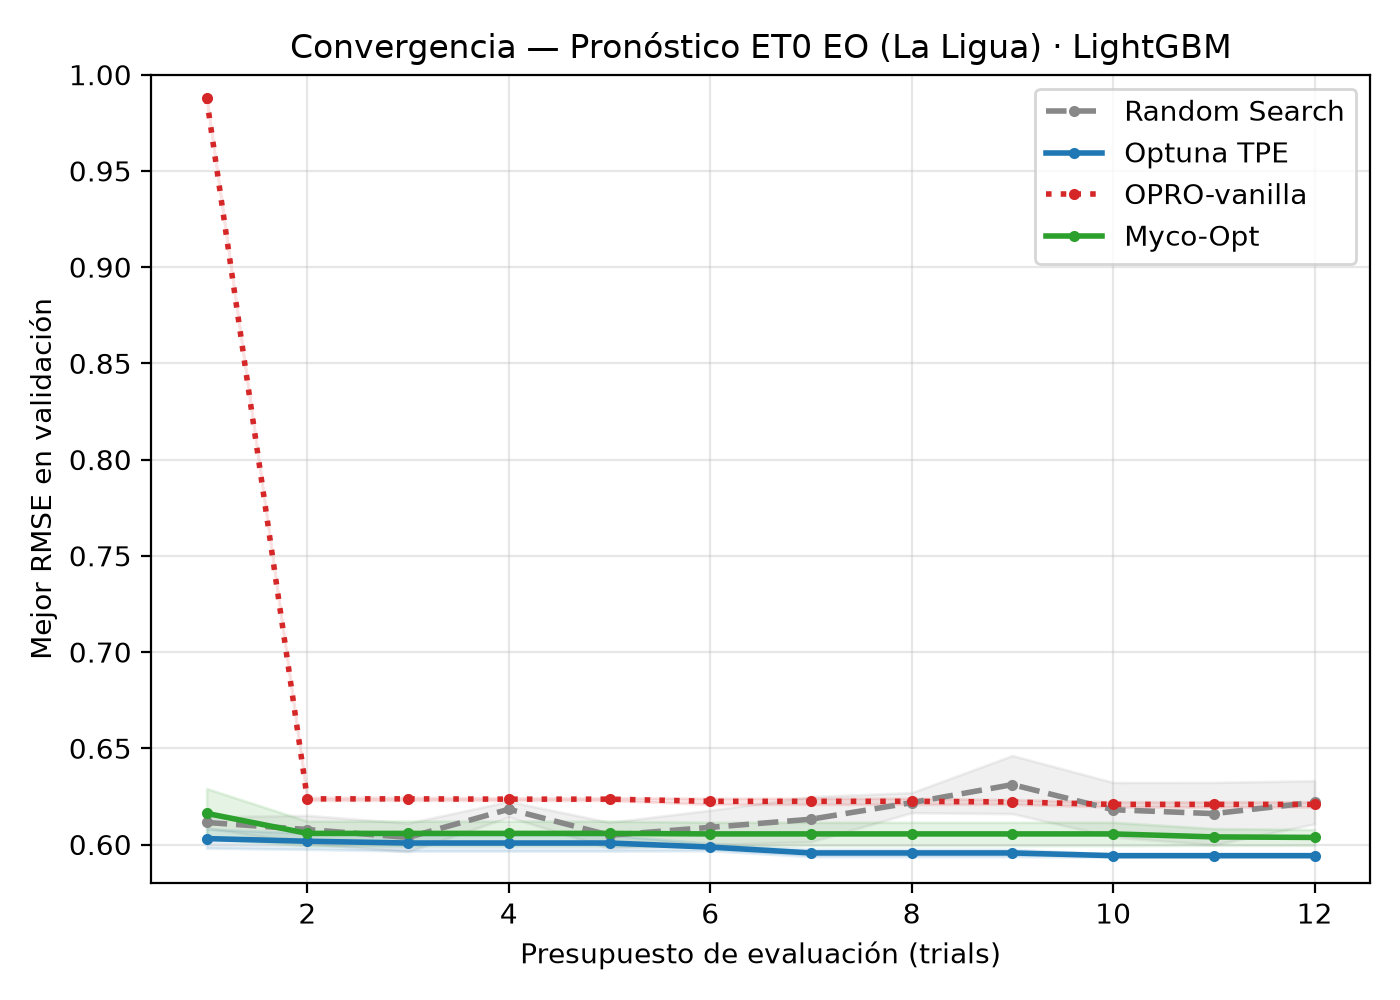
\includegraphics[width=0.78\columnwidth]{../figures/fig1_convergencia.png}
\caption{Convergence of the four methods on validation (mean over 3 seeds,
shaded = $\pm$1 std). The unconstrained LLM (OPRO-vanilla) starts poorly and
plateaus high; the mycorrhizal prior (Myco-Opt) starts competitive and
converges faster. Classical TPE remains the strongest baseline at this budget.}
\label{fig:convergence}
\end{figure}

\textbf{The prior is what makes the LLM optimizer work.} At the \emph{first}
evaluation (the pure prior, before feedback), OPRO-vanilla's proposal has
validation RMSE 0.988 across seeds, whereas Myco-Opt's first proposal averages
0.616 (0.598 best seed). After 12 trials, unconstrained OPRO converges to
0.621 --- \emph{still worse than Myco-Opt's very first proposal}. The prior
compresses the search space into the statistically plausible region, exactly
what a scarce-budget regime needs.

Classical TPE remains the strongest method at this budget (test RMSE 0.606
vs.\ 0.614) --- when each evaluation costs under a second, TPE's surrogate
amortizes quickly; the regime where Myco-Opt's advantage is structural is the
\emph{expensive-evaluation} regime of neural EO pipelines (Section~\ref{sec:discussion}).

\section{Discussion and limitations}
\label{sec:discussion}

OPRO-vanilla and Myco-Opt differ only in the prior constraining proposal
ranges; the consistent improvement (test RMSE 0.627 $\rightarrow$ 0.614;
first-trial 0.988 $\rightarrow$ 0.616) shows that \emph{quantitative
biological topology transfers} into useful inductive bias for LLM-based HPO.
Limitations: classical BO still wins at cheap budgets (the prior's advantage
grows with evaluation cost); we use one network and one EO task (follow-up will
use GlobalFungi \citep{vetrovsky2020} and neural EO models); the
topology-to-hyperparameter mapping is interpretable but partly heuristic; and
we use only measured statistics, acknowledging the critique of
common-mycorrhizal-network inference \citep{karst2023}. Aligned with this workshop's
open-infrastructure emphasis, all code, data and the prior will be released
open source.

\section{Conclusion and future work}
\label{sec:conclusion}

We presented Myco-Opt, an LLM-driven HPO optimizer whose search space is
constrained by metrics measured on a real mycorrhizal network. On an
agricultural EO benchmark (daily ET$_0$ forecasting for avocado orchards in
drought-stricken Chile), the prior turned an unconstrained LLM that plateaus at
RMSE 0.627 into one reaching 0.614 at the same budget --- with a first proposal
(0.616) beating the unconstrained LLM's converged result. Classical TPE remains
the reference at cheap budgets; Myco-Opt's promise lies in expensive-evaluation
regimes, to be validated with neural pipelines. We aim to seed discussion of
\emph{biological inductive biases for AutoML in EO}.

% ==== Bibliography
\bibliography{references}

\end{document}
